\documentclass{article}

\usepackage{addfont} % for new fonts
    \addfont{OT1}{d7seg}{\dviiseg}

\usepackage{amsmath}

\usepackage{array} % for \setextrarowheight and \multicolumn

\usepackage{geometry} %for formatting
    \geometry{a4paper,landscape=True,layoutsize={29.7cm,21cm},layoutoffset={0cm,0cm},showcrop,textwidth=27.7cm,textheight=19cm}  
    
\usepackage{graphicx} % For inserting images.

\usepackage{tikz} % For creating tikz images.

\usepackage{titlesec} % For title modification
    \renewcommand{\thesection}{\hspace*{-1.0em}} % No numbering for section titles

\setlength\parindent{0pt} % For no indent at paragraph beginning.

\title{Reporting Measurements}
\author{BBB}
\date{2025}

\begin{document}

\pagestyle{empty} % no numbering or smt on page

\centering

\setlength\extrarowheight{3pt}

\begin{minipage}[t][18cm][c]{11cm}


\section{\Huge Reporting Measurements}


A measurement of any \textbf{quantity} $f$ is typically reported like
\begin{align*}
    f & = (3.14 \pm 0.15) \cdot 10^9 \: \text{m},
\end{align*}
a \textbf{value} ($3.14 \cdot 10^9 \: \text{m}$) and a non-zero positive \textbf{uncertainty} ($0.15 \cdot 10^9 \: \text{m}$). These have the same \textbf{unit} ($\text{m}$) and are \textbf{rounded} to the same place (0.01), typically such that the uncertainty has 1 or 2 \textbf{significant digits}.\bigskip


\begin{itemize}
    \item If $f$ is directly measured once, then this value is reported and the uncertainty is an estimate: If the instrument does not list one, then you may use its resolution, or, for a ruler, half of its resolution.
\end{itemize}
\begin{centering}
    \begin{minipage}{6cm}
        \centering
        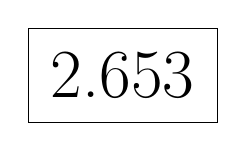
\begin{tikzpicture}
            \draw [draw=black] (-1.2,-0.6) rectangle (1.2,0.6);
            \draw node at (0,0) {\Huge\dviiseg 2.653};
        \end{tikzpicture}\\
        $f = (2.653 \pm 0.001) \: \text{A}$
    \end{minipage}
    \begin{minipage}{5cm}
        \centering
        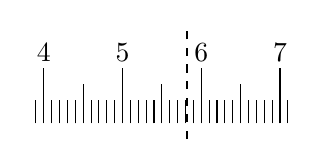
\begin{tikzpicture}
            \draw (-1.6,0) -- (-1.6,0.3);
            \draw (-1.5,0) -- (-1.5,0.7);
            \draw node at (-1.5,0.9) {4};
            \draw (-1.4,0) -- (-1.4,0.3);
            \draw (-1.3,0) -- (-1.3,0.3);
            \draw (-1.2,0) -- (-1.2,0.3);
            \draw (-1.1,0) -- (-1.1,0.3);
            \draw (-1.2,0) -- (-1.2,0.3);
            \draw (-1.1,0) -- (-1.1,0.3);
            \draw (-1  ,0) -- (-1  ,0.5);
            \draw (-0.9,0) -- (-0.9,0.3);
            \draw (-0.8,0) -- (-0.8,0.3);
            \draw (-0.7,0) -- (-0.7,0.3);
            \draw (-0.6,0) -- (-0.6,0.3);
            \draw (-0.5,0) -- (-0.5,0.7);
            \draw node at (-0.5,0.9) {5};
            \draw (-0.4,0) -- (-0.4,0.3);
            \draw (-0.3,0) -- (-0.3,0.3);
            \draw (-0.2,0) -- (-0.2,0.3);
            \draw (-0.1,0) -- (-0.1,0.3);
            \draw ( 0  ,0) -- ( 0  ,0.5);
            \draw ( 0.1,0) -- ( 0.1,0.3);
            \draw ( 0.2,0) -- ( 0.2,0.3);
            \draw ( 0.3,0) -- ( 0.3,0.3);
            \draw[dashed,thick] (0.32,-0.2) -- ( 0.32,1.2);
            \draw ( 0.4,0) -- ( 0.4,0.3);
            \draw ( 0.5,0) -- ( 0.5,0.7);
            \draw node at ( 0.5,0.9) {6};
            \draw ( 0.6,0) -- ( 0.6,0.3);
            \draw ( 0.7,0) -- ( 0.7,0.3);
            \draw ( 0.8,0) -- ( 0.8,0.3);
            \draw ( 0.9,0) -- ( 0.9,0.3);
            \draw ( 1  ,0) -- ( 1  ,0.5);
            \draw ( 1.1,0) -- ( 1.1,0.3);
            \draw ( 1.2,0) -- ( 1.2,0.3);
            \draw ( 1.3,0) -- ( 1.3,0.3);
            \draw ( 1.4,0) -- ( 1.4,0.3);
            \draw ( 1.5,0) -- ( 1.5,0.7);
            \draw node at ( 1.5,0.9) {7};
            \draw ( 1.6,0) -- ( 1.6,0.3);
        \end{tikzpicture}\\
        $f = (5.80 \pm 0.05) \: \text{cm}$
    \end{minipage}
\end{centering}

\begin{itemize}
    \item If $f$ is directly measured $M \gg 1$ times (significantly more than once), then the value is the \textbf{estimated} \textbf{mean} and the uncertainty is $1/\sqrt{M}$ times the \textbf{estimated} \textbf{standard deviation}.
\end{itemize}
\begin{itemize}
    \item If $f$ is calculated from 1 or more independent quantities with values $x_i$ and uncertainties $\Delta x_i$, then the value is a function $f(x_i)$ and the uncertainty $\Delta f$ is calculated by \textbf{uncertainty propagation}.
\end{itemize}


\begin{tabular}{|m{0.35\textwidth}|m{0.55\textwidth}|}
    \hline
    \textbf{Function} & \textbf{Gaussian uncertainty propagation}\\
    \hline
    $f(x_i)$ differentiable &  $\Delta f = \sqrt{\sum_{j} \left( \frac{\partial f(x_i)}{\partial x_j} \Delta x_j \right)^2}$ \\
    & All cases below follow from this one.\\
    \hline
    $f = x_1 + x_2$ or $x_1 - x_2$ & $\Delta f = \sqrt{(\Delta x_1)^2 + (\Delta x_2)^2}$\\
    \hline
    $f = x_1x_2$ or $x_1 / x_2$ & $\Delta f = \left|f\right| \sqrt{(\Delta x_1 / x_1)^2 + (\Delta x_2/x_2)^2}$\\
    \hline    
    $f = cx$ & $\Delta f = \left|c\right| \Delta x$ \\
    \hline
    $f = x^c$ & $\Delta f = \left|f \: c \: \Delta x / x \right|$\\
    \hline
    $f = \overline{x} = (\sum_{i=1}^M x_i)/M $ & $\Delta f = \sqrt{\sum_{i=1}^M (\Delta x_i)^2} / M \approx \sigma_x / \sqrt{M}$ \\
    \hline
\end{tabular}

\bigskip

For deeper insight, you may look into \textbf{random variables}, the \textbf{Gaussian distribution}, the \textbf{central limit theorem} and \textbf{confidence intervalls}. 


\end{minipage}
\begin{minipage}[t][18cm][c]{0.5cm}
    \hfill
\end{minipage}
\begin{minipage}[t][18cm][c]{13cm}
    \centering

    \begin{tabular}{|m{0.83\textwidth}|}    
        \hline
        \begin{tabular}{l|l}
            \textbf{Uncertainty} & \textbf{Error} \\
            \hline
            \textbf{Statistical} deviation from true
            & \textbf{Systematic} deviation from true\\
             value. Gets smaller with $1/\sqrt{M}$. 
            &  value. Independent of $M$. \\
        \end{tabular}\\
        
        \hline
        
        \begin{centering}
            \begin{tabular}{cc}
                \textbf{precise} = smaller uncertainty & \textbf{accurate} = smaller error \\
                \textbf{imprecise} = larger uncertainty & \textbf{inaccurate} = larger error\\
            \end{tabular}\\ 
            \smallskip
            \begin{minipage}[t]{2cm}
                \centering
                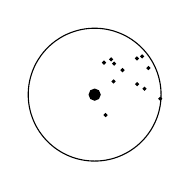
\begin{tikzpicture}
                    \draw[black] (0,0) circle (24pt);
                    \draw[fill=black] (0,0) circle (2pt);
                    \draw[fill=black] (15.355134405361072pt,3.79418712320912pt) circle (.5pt);
                    \draw[fill=black] (6.8409046722809235pt,4.776970250490139pt) circle (.5pt);
                    \draw[fill=black] (18.01765674378749pt,2.141272645171564pt) circle (.5pt);
                    \draw[fill=black] (5.941468062565262pt,12.758896892467408pt) circle (.5pt);
                    \draw[fill=black] (10.060092661935546pt,8.868953575919729pt) circle (.5pt);
                    \draw[fill=black] (3.3810861018466483pt,11.563133989501196pt) circle (.5pt);
                    \draw[fill=black] (19.42511882780015pt,9.61967349056972pt) circle (.5pt);
                    \draw[fill=black] (3.950171095165434pt,-7.371801599852983pt) circle (.5pt);
                    \draw[fill=black] (7.0238362222184865pt,11.216690771575028pt) circle (.5pt);
                    \draw[fill=black] (23.71866212150824pt,-1.4702304804314208pt) circle (.5pt);
                    \draw[fill=black] (15.291639269634945pt,13.085154162432783pt) circle (.5pt);
                    \draw[fill=black] (17.156842008139122pt,13.801535756592525pt) circle (.5pt);
                \end{tikzpicture}\newline
                imprecise\newline
                inaccurate
            \end{minipage}
            \begin{minipage}[t]{2cm}
                \centering
                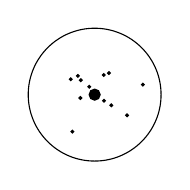
\begin{tikzpicture}
                    \draw[black] (0,0) circle (24pt);
                    \draw[fill=black] (0,0) circle (2pt);
                    \draw[fill=black] (3.3551344053610723pt,-2.20581287679088pt) circle (.5pt);
                    \draw[fill=black] (-5.1590953277190765pt,-1.2230297495098612pt) circle (.5pt);
                    \draw[fill=black] (6.017656743787493pt,-3.858727354828436pt) circle (.5pt);
                    \draw[fill=black] (-6.058531937434738pt,6.758896892467408pt) circle (.5pt);
                    \draw[fill=black] (-1.939907338064454pt,2.8689535759197287pt) circle (.5pt);
                    \draw[fill=black] (-8.618913898153352pt,5.563133989501195pt) circle (.5pt);
                    \draw[fill=black] (17.42511882780015pt,3.6196734905697197pt) circle (.5pt);
                    \draw[fill=black] (-8.049828904834566pt,-13.371801599852983pt) circle (.5pt);
                    \draw[fill=black] (-4.9761637777815135pt,5.216690771575028pt) circle (.5pt);
                    \draw[fill=black] (11.718662121508238pt,-7.470230480431421pt) circle (.5pt);
                    \draw[fill=black] (3.291639269634945pt,7.085154162432783pt) circle (.5pt);
                    \draw[fill=black] (5.156842008139121pt,7.801535756592525pt) circle (.5pt);
                \end{tikzpicture}\newline
                imprecise\newline
                accurate
            \end{minipage}
            \begin{minipage}[t]{2cm}
                \centering
                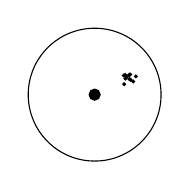
\begin{tikzpicture}
                    \draw[black] (0,0) circle (24pt);
                    \draw[fill=black] (0,0) circle (2pt);
                    \draw[fill=black] (12.55918906756018pt,5.632364520534853pt) circle (.5pt);
                    \draw[fill=black] (11.140150778713487pt,5.796161708415023pt) circle (.5pt);
                    \draw[fill=black] (13.002942790631248pt,5.356878774195261pt) circle (.5pt);
                    \draw[fill=black] (10.99024467709421pt,7.126482815411235pt) circle (.5pt);
                    \draw[fill=black] (11.676682110322592pt,6.478158929319955pt) circle (.5pt);
                    \draw[fill=black] (10.563514350307775pt,6.927188998250199pt) circle (.5pt);
                    \draw[fill=black] (14.904186471300026pt,6.603278915094953pt) circle (.5pt);
                    \draw[fill=black] (10.65836184919424pt,3.771366400024503pt) circle (.5pt);
                    \draw[fill=black] (11.170639370369749pt,6.869448461929172pt) circle (.5pt);
                    \draw[fill=black] (13.953110353584707pt,4.754961586594764pt) circle (.5pt);
                    \draw[fill=black] (12.548606544939158pt,7.18085902707213pt) circle (.5pt);
                    \draw[fill=black] (12.859473668023186pt,7.3002559594320875pt) circle (.5pt);
                \end{tikzpicture}\newline
                precise\newline
                inaccurate
            \end{minipage}
            \begin{minipage}[t]{2cm}
                \centering
                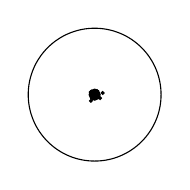
\begin{tikzpicture}
                    \draw[black] (0,0) circle (24pt);
                    \draw[fill=black] (0,0) circle (2pt);
                    \draw[fill=black] (0.5591890675601787pt,-0.36763547946514663pt) circle (.5pt);
                    \draw[fill=black] (-0.8598492212865128pt,-0.20383829158497688pt) circle (.5pt);
                    \draw[fill=black] (1.0029427906312487pt,-0.6431212258047393pt) circle (.5pt);
                    \draw[fill=black] (-1.0097553229057896pt,1.1264828154112347pt) circle (.5pt);
                    \draw[fill=black] (-0.323317889677409pt,0.4781589293199548pt) circle (.5pt);
                    \draw[fill=black] (-1.4364856496922251pt,0.9271889982501992pt) circle (.5pt);
                    \draw[fill=black] (2.9041864713000254pt,0.6032789150949532pt) circle (.5pt);
                    \draw[fill=black] (-1.341638150805761pt,-2.228633599975497pt) circle (.5pt);
                    \draw[fill=black] (-0.8293606296302523pt,0.8694484619291712pt) circle (.5pt);
                    \draw[fill=black] (1.9531103535847063pt,-1.2450384134052368pt) circle (.5pt);
                    \draw[fill=black] (0.5486065449391575pt,1.1808590270721304pt) circle (.5pt);
                    \draw[fill=black] (0.8594736680231868pt,1.3002559594320875pt) circle (.5pt);
                \end{tikzpicture}\newline
                precise\newline
                accurate
            \end{minipage}\\
        \end{centering}\\
        \hline
        Beware: Many people use \textit{uncertainty} and \textit{error} interchangeably, or \textit{statistical error} for uncertainty, or \textit{systematic uncertainty} for error.
        \smallskip\\
        \hline
    \end{tabular}

    
    \vfill
    \begin{tabular}{|m{0.4\textwidth}|m{0.4\textwidth}|}
        \hline
        \textbf{Mean}
        & \textbf{Standard deviation}\\
        \hline
        \multicolumn{2}{|m{0.8\textwidth}|}{
            \hspace{-0.6cm} Let there be a \textbf{sample}, any set of $M \geq 2$ values $f_i$ randomly drawn from a \textbf{population}, any set of $N>M$ values $g_i$.
        }\\
        \hline
        Mean of population\newline
        $\overline{g} = (\sum_{i=1}^N g_i)/N$ 
        &
        Standard deviation of population\newline
        $\sigma_g = \sqrt{\sum_{i=1}^N \left(g_i-\overline{g}\right)^2}/ \sqrt{N}$
        \\  
        \textbf{Estimated mean}\newline
        $\overline{g} \approx (\sum_{i=1}^M f_i)/M = \overline{f}$
        &
        \textbf{Estimated standard deviation}\newline
        $\sigma_g \approx \sqrt{\sum_{i=1}^M \left(f_i-\overline{f}\right)^2}/ \sqrt{M-1}$
        \\
        & 
        This underestimates $\sigma_g$. Would be unbiased with both sides squared.
        \\
        \hline
    \end{tabular}
    
    \vfill

    \begin{tabular}{|m{0.4\textwidth}|m{0.4\textwidth}|}
        \hline
        \textbf{Rounding half up} & \textbf{Gaussian rounding} \\
        \hline
        For equally near options, choose the larger one.
        &
        For equally near options, choose the one whose last digit is even.
        \\
        \hline
        $
        \begin{aligned}
            && 1.4999 & \approx 1 &&&&& 2.4999 & \approx 2 &&\\
            && 1.5 & \approx 2 &&&&& \textbf{2.5} & \approx \textbf{3} &&\\
            && 1.5001 & \approx 2 &&&&& 2.5001 & \approx 3 &&
        \end{aligned}
        $ 
        \smallskip
        &
        $
        \begin{aligned}
            && 1.4999 & \approx 1 &&&&& 2.4999 & \approx 2 &&\\
            && 1.5 & \approx 2 &&&&& \textbf{2.5} & \approx \textbf{2} &&\\
            && 1.5001 & \approx 2 &&&&& 2.5001 & \approx 3 &&
        \end{aligned}
        $
        \smallskip\\
        \hline   
        Biases towards larger numbers. The mean of rounded uniformly drawn numbers is biased. Often taught in school.
        \smallskip
        &
        Biases towards even last digits. The mean of rounded uniformly drawn numbers is unbiased. \text{Often} preferred by scientists.
        \smallskip\\
        \hline
    \end{tabular}
\end{minipage}
















\end{document}
